\chapter{Confusion and $\epsilon^{i,\gamma\gamma}_k$ matrices: \Hgg}\label{app:eff_acc}
This Appendix contains the confusion matrix for the full set of analysis categories used in the \Hgg analysis. This differs from Figure~\ref{fig:purity_matrix} as the categories are fully split into the individual tags. Moreover, the detector efficiency times analysis acceptance terms, $\epsilon^{i,\gamma\gamma}_{k}$, used in the normalisation of the signal models are shown. These terms are derived separately for the 2016, 2017, and 2018 simulation.


\begin{figure}
  \centering
  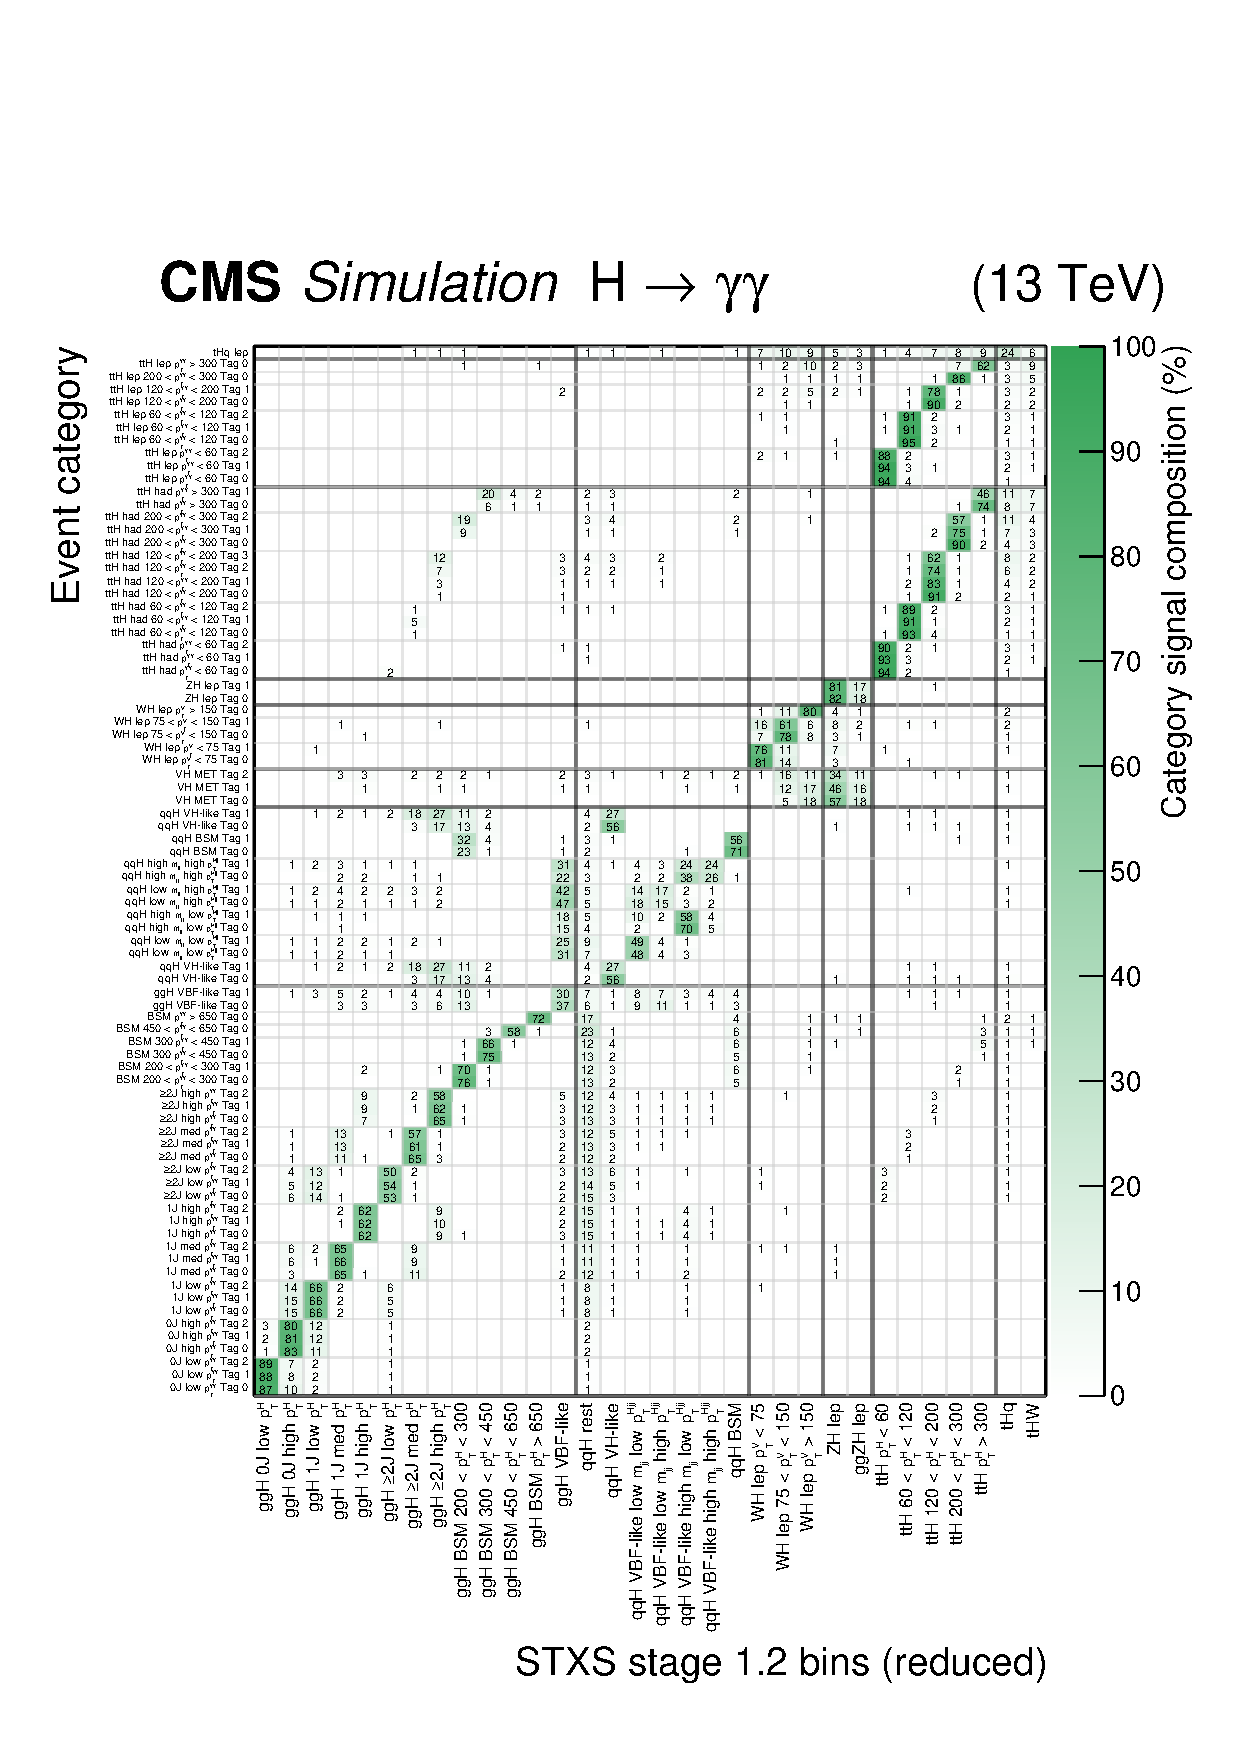
\includegraphics[width=1\textwidth]{Figures/app_matrices/purityMatrix_thesis.pdf}
  \caption[Confusion matrix for the full set of analysis categories]
  {
    Confusion matrix displaying the composition of each analysis category in terms of a merged set of STXS bins. The colour scale corresponds to the fractional yield in each analysis category (row), accounted for by each STXS process (column). Each row therefore sums to 100\%. Entries with values less than 0.5\% are not shown. Simulated events for each year in the period 2016-2018 are combined with appropriate weights corresponding to their relative integrated luminosity in data. The column labelled as qqH rest includes the contributions from the qqH 0J, qqH 1J, qqH $m_{jj}<60$~GeV and the qqH $120<m_{jj}<350$~GeV STXS bins.
  }
  \label{fig:purity_matrix_full}
\end{figure}

\begin{figure}
  \centering
  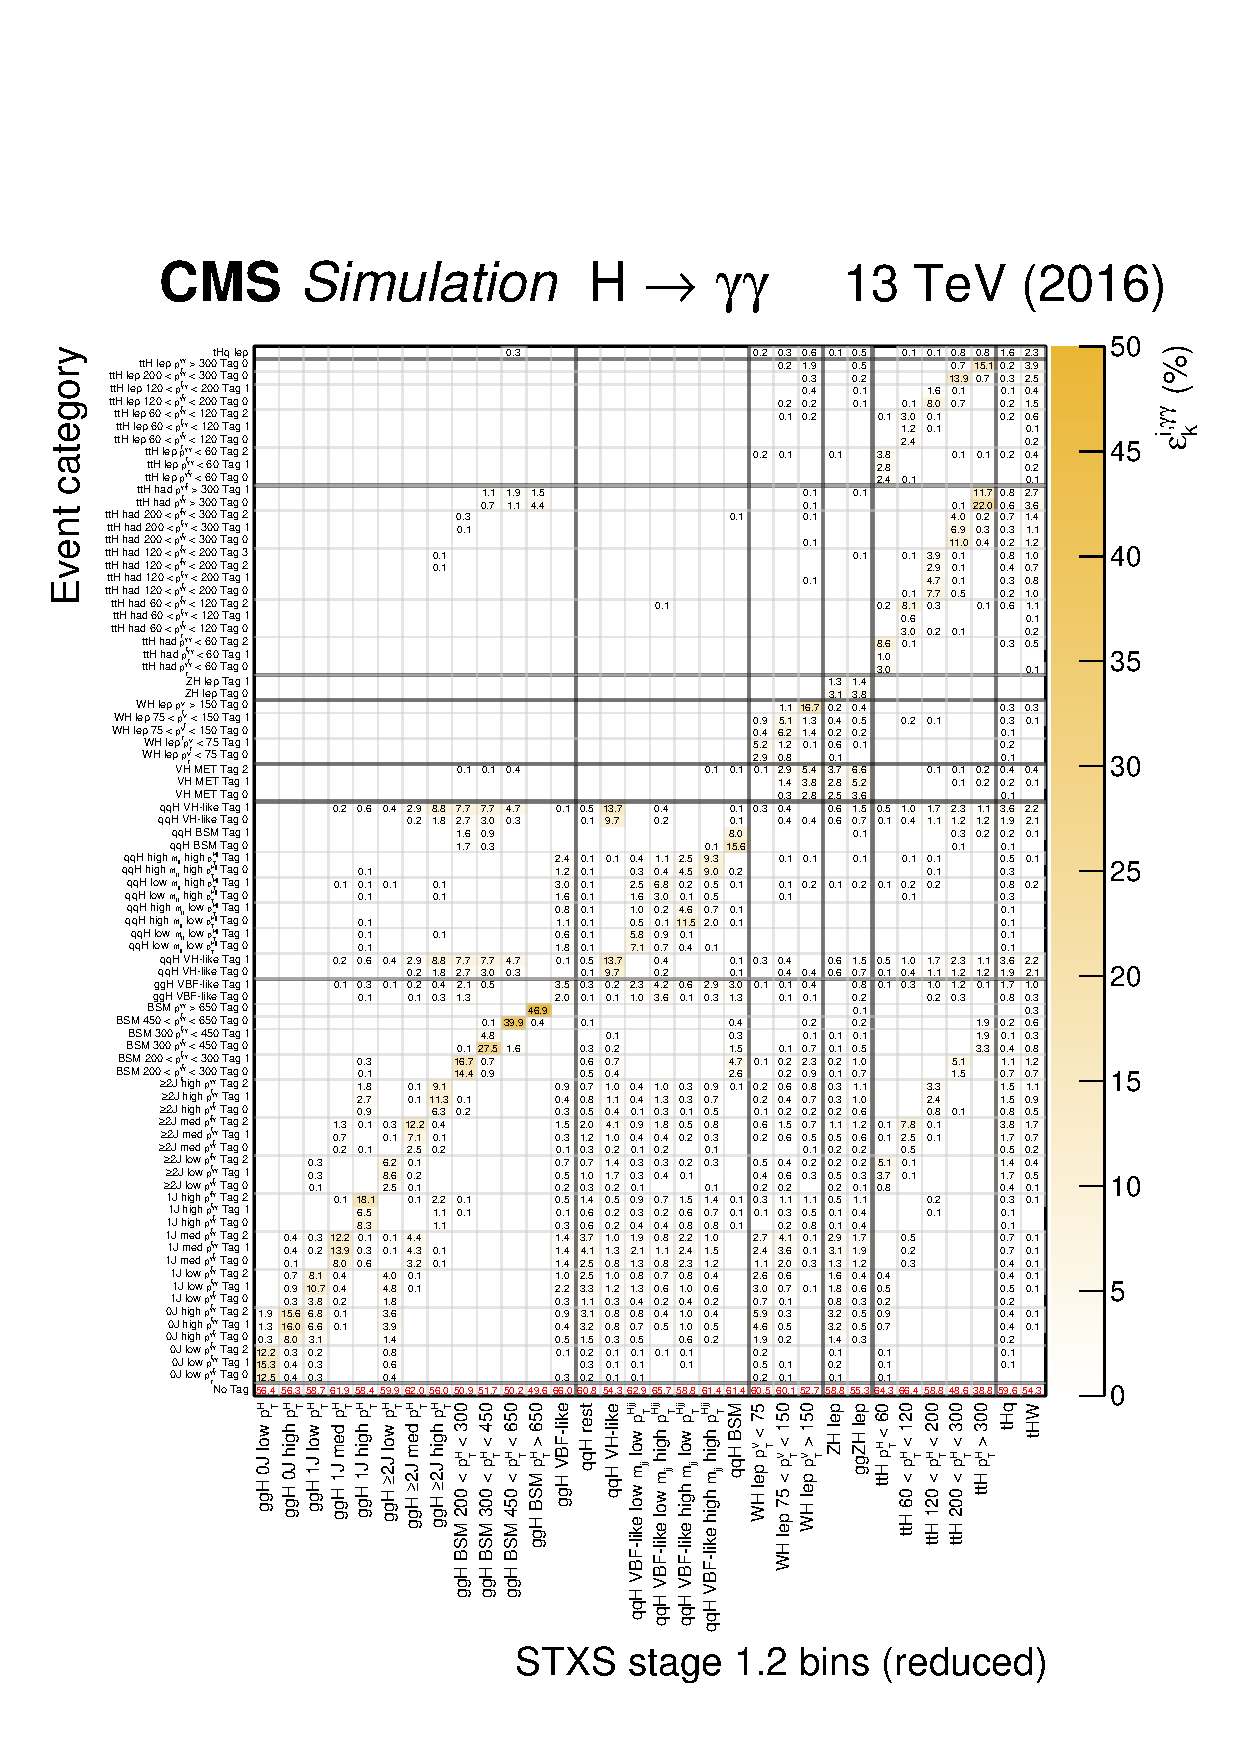
\includegraphics[width=1\textwidth]{Figures/app_matrices/migrationMatrix_2016_thesis.pdf}
  \caption[Efficiency times acceptance matrix from 2016 simulation]
  {
    A matrix showing the $\epsilon^{i,\gamma\gamma}_{k}$ terms for a merged set of STXS bins, derived from 2016 simulation. The bin merging is done purely for plotting purposes; in the analysis a separate $\epsilon^{i,\gamma\gamma}_{k}$ factor is calculated for each STXS bin. The numbers show the fraction of the total yield of each (merged) STXS bin, landing in each analysis category. Each column therefore sums to 100\%. Entries with values less than 0.05\% are not shown. The bottom row, referred to as ``No Tag" indicates the fraction of events originating from the corresponding process which do not enter a single analysis category. The column labelled as qqH rest includes the contributions from the qqH 0J, qqH 1J, qqH $m_{jj}<60$~GeV and the qqH $120<m_{jj}<350$~GeV STXS bins.
  }
  \label{fig:ea_2016}
\end{figure}

\begin{figure}
  \centering
  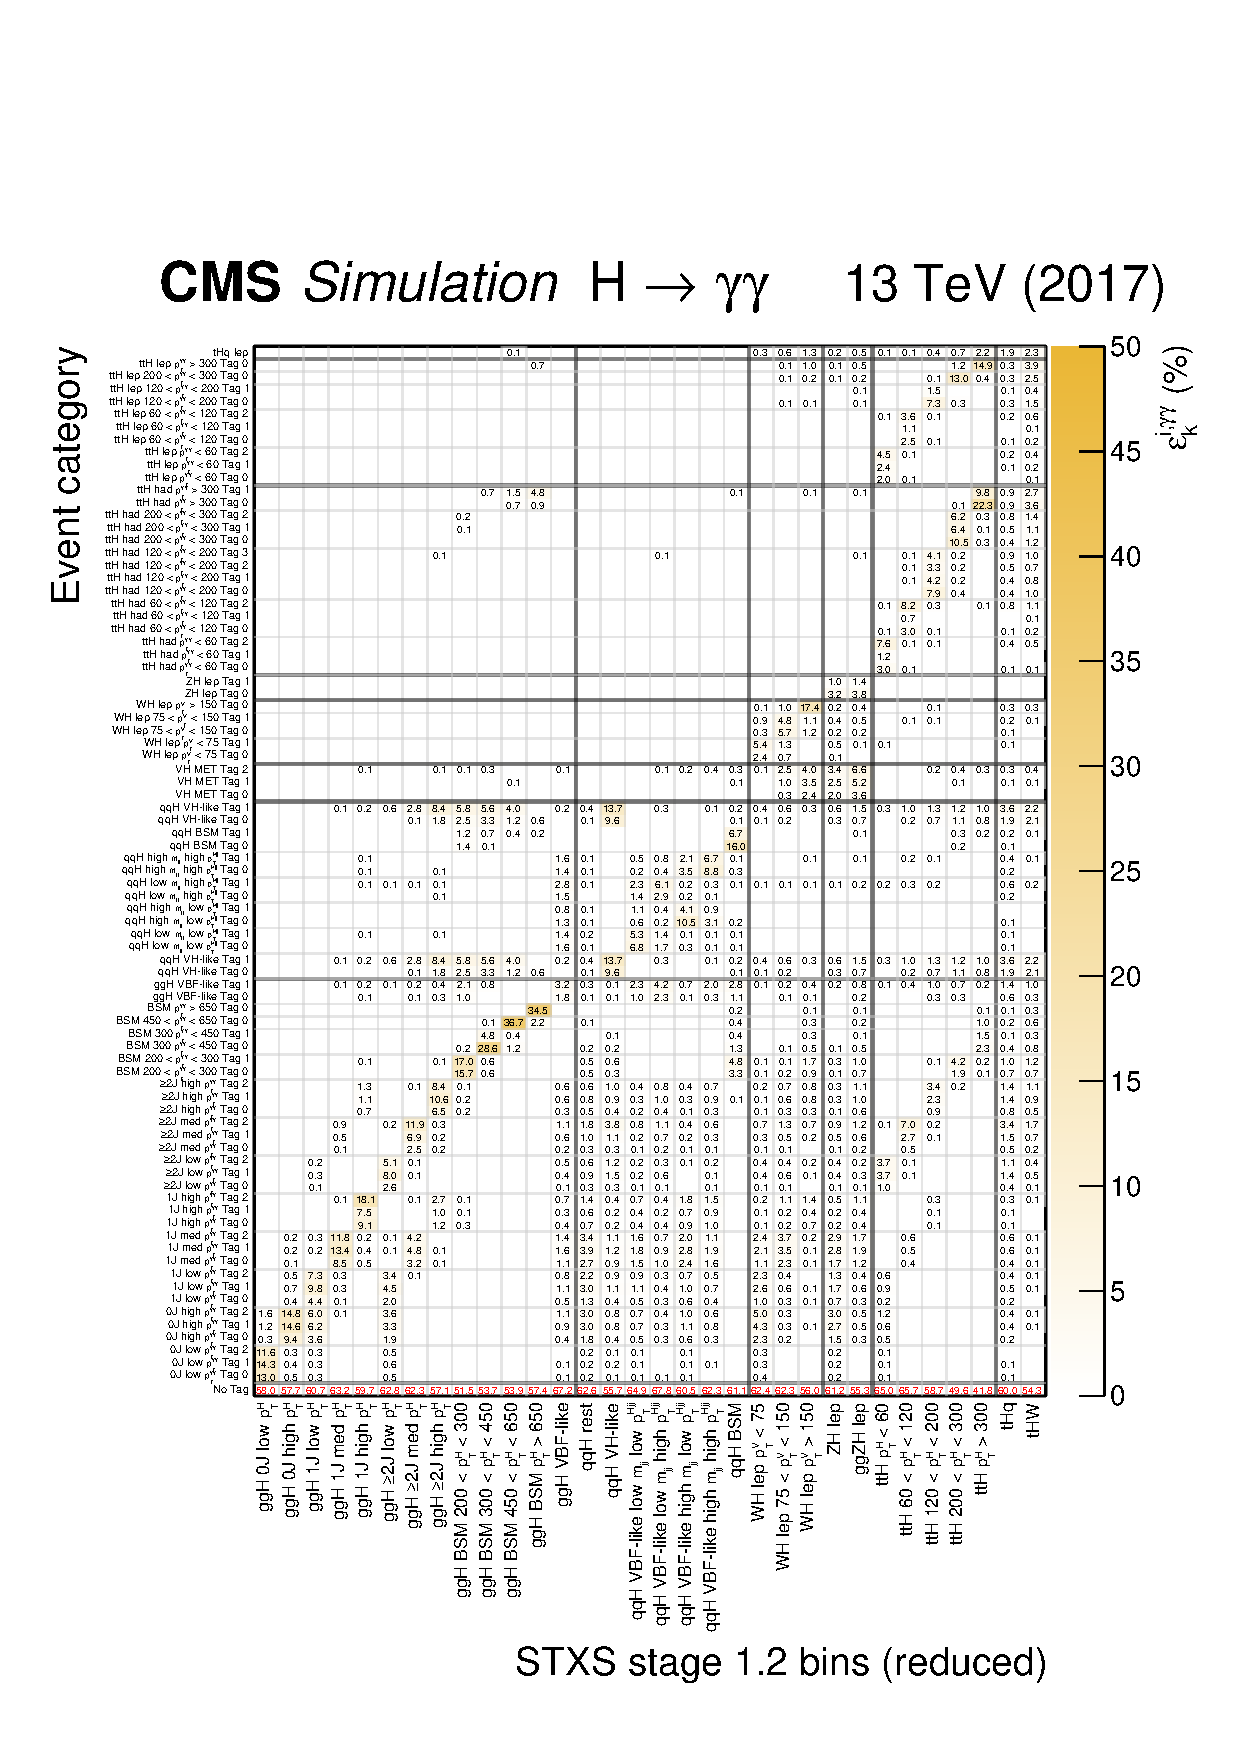
\includegraphics[width=1\textwidth]{Figures/app_matrices/migrationMatrix_2017_thesis.pdf}
  \caption[Efficiency times acceptance matrix from 2017 simulation]
  {
    A matrix showing the $\epsilon^{i,\gamma\gamma}_{k}$ terms for a merged set of STXS bins, derived from 2017 simulation. The bin merging is done purely for plotting purposes; in the analysis a separate $\epsilon^{i,\gamma\gamma}_{k}$ factor is calculated for each STXS bin. The numbers show the fraction of the total yield of each (merged) STXS bin, landing in each analysis category. Each column therefore sums to 100\%. Entries with values less than 0.05\% are not shown. The bottom row, referred to as ``No Tag" indicates the fraction of events originating from the corresponding process which do not enter a single analysis category. The column labelled as qqH rest includes the contributions from the qqH 0J, qqH 1J, qqH $m_{jj}<60$~GeV and the qqH $120<m_{jj}<350$~GeV STXS bins.
  }
  \label{fig:ea_2017}
\end{figure}

\begin{figure}
  \centering
  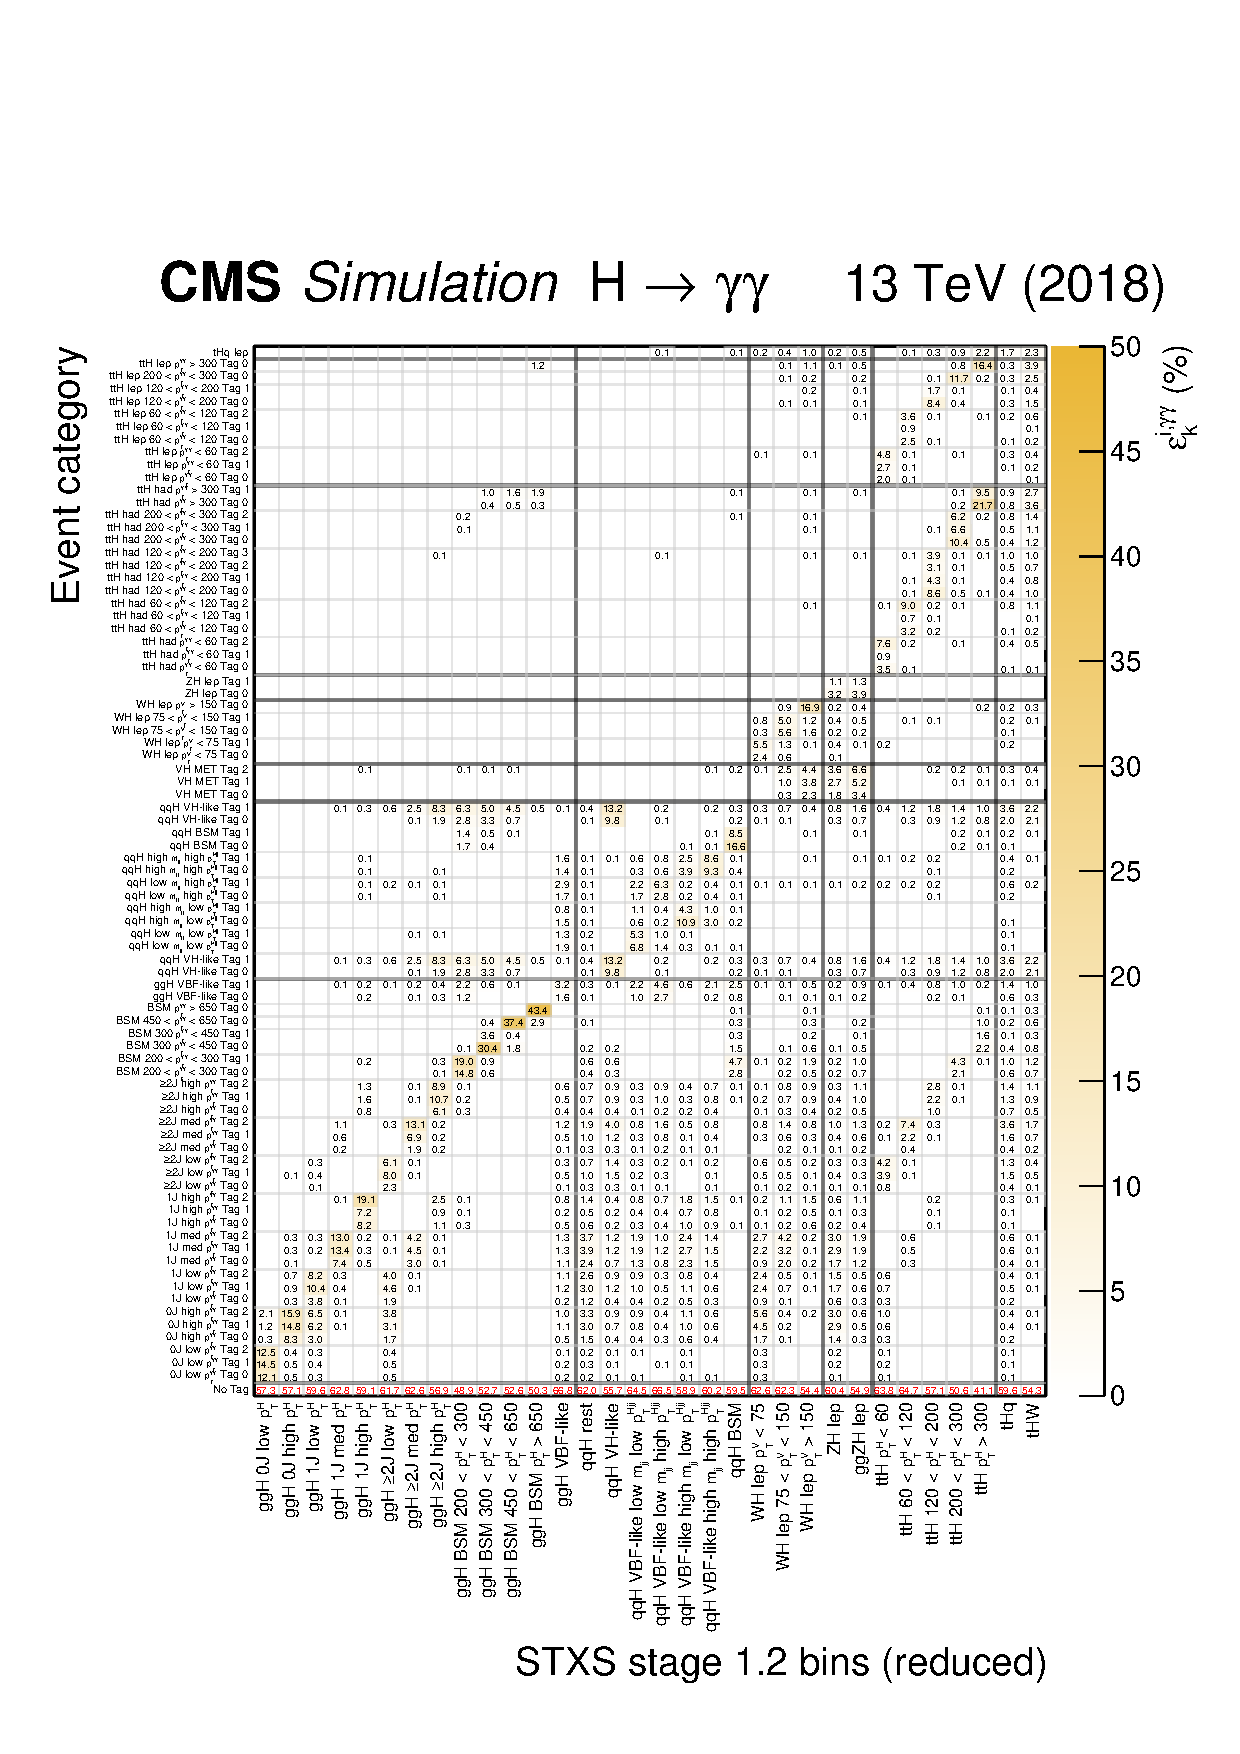
\includegraphics[width=1\textwidth]{Figures/app_matrices/migrationMatrix_2018_thesis.pdf}
  \caption[Efficiency times acceptance matrix from 2018 simulation]
  {
    A matrix showing the $\epsilon^{i,\gamma\gamma}_{k}$ terms for a merged set of STXS bins, derived from 2018 simulation. The bin merging is done purely for plotting purposes; in the analysis a separate $\epsilon^{i,\gamma\gamma}_{k}$ factor is calculated for each STXS bin. The numbers show the fraction of the total yield of each (merged) STXS bin, landing in each analysis category. Each column therefore sums to 100\%. Entries with values less than 0.05\% are not shown. The bottom row, referred to as ``No Tag" indicates the fraction of events originating from the corresponding process which do not enter a single analysis category. The column labelled as qqH rest includes the contributions from the qqH 0J, qqH 1J, qqH $m_{jj}<60$~GeV and the qqH $120<m_{jj}<350$~GeV STXS bins.
  }
  \label{fig:ea_2017}
\end{figure}